\section{Error Analysis of Structured Light}
\frame{
  \frametitle{An Error Analysis of Structured Light Scanning of Biological Tissue}
  Sebastian Nesgaard Jensen, Jakob Wilm, Henrik Aanæs

  \textit{SCIA 2017}
  \begin{figure}
    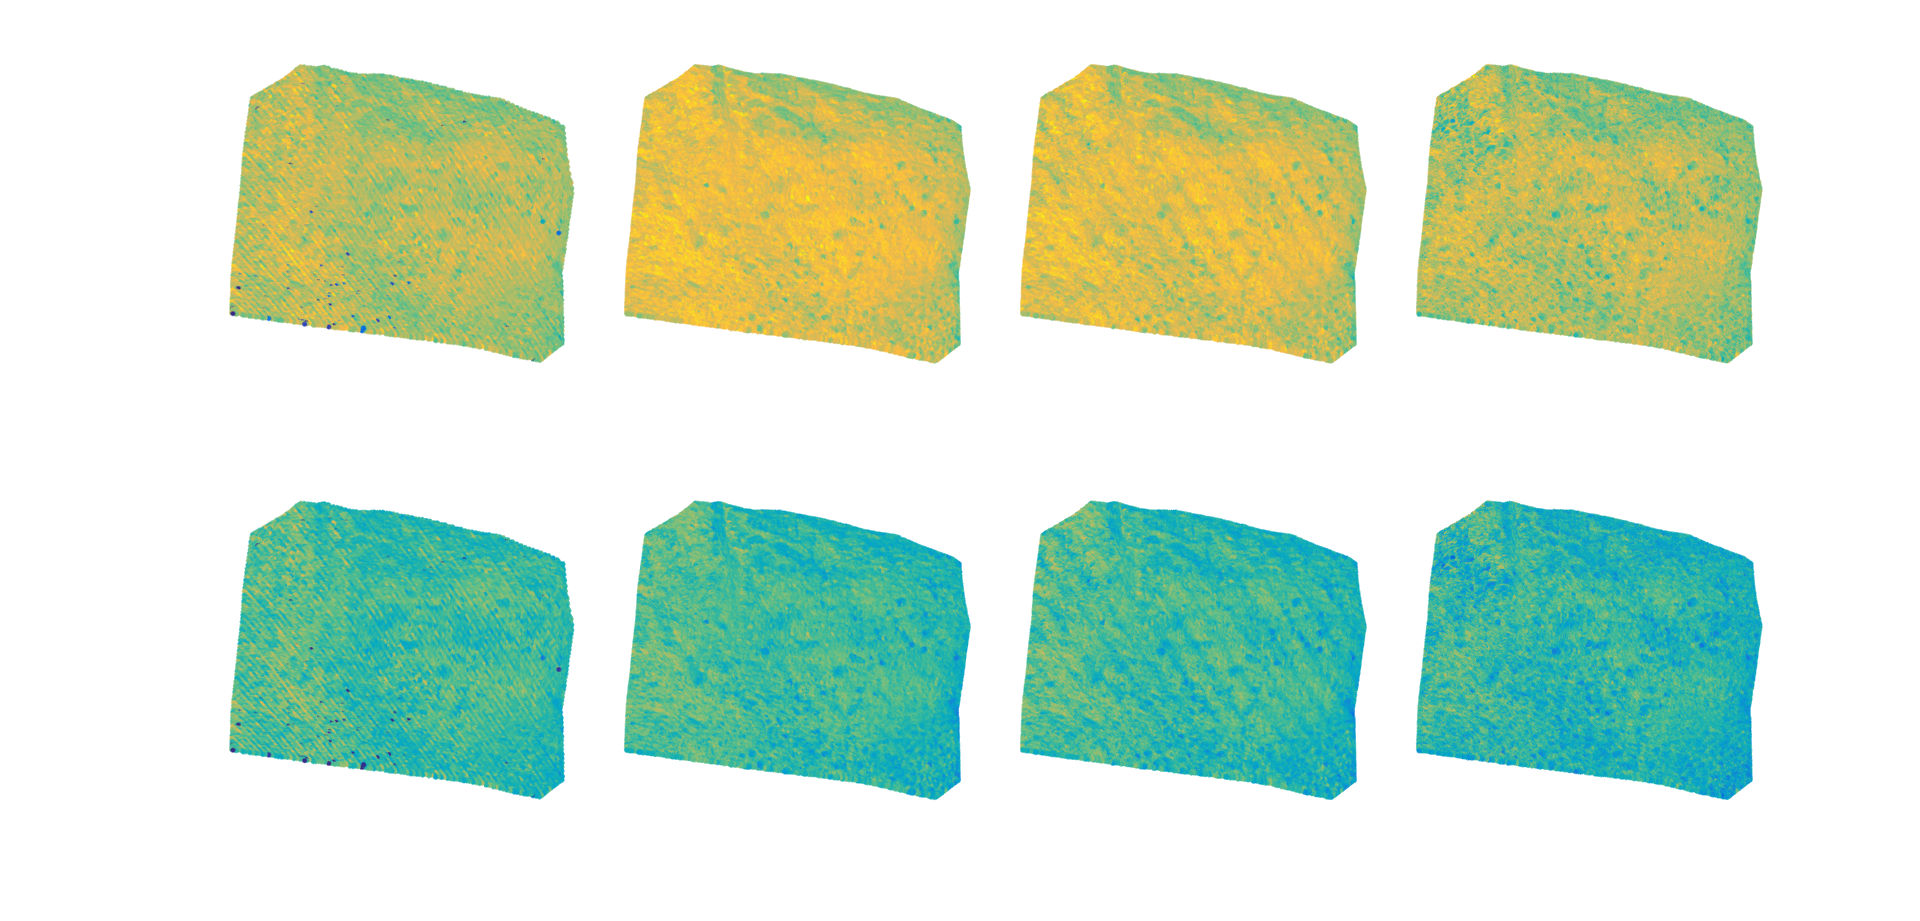
\includegraphics[width=0.80\linewidth]{figures/stlmeat}
      \hfill
  \end{figure}
  %\bibentry{jensen2017error}
}

\frame{
  \frametitle{Camera-Projector Structured Light}
  \begin{figure}
    \centering
    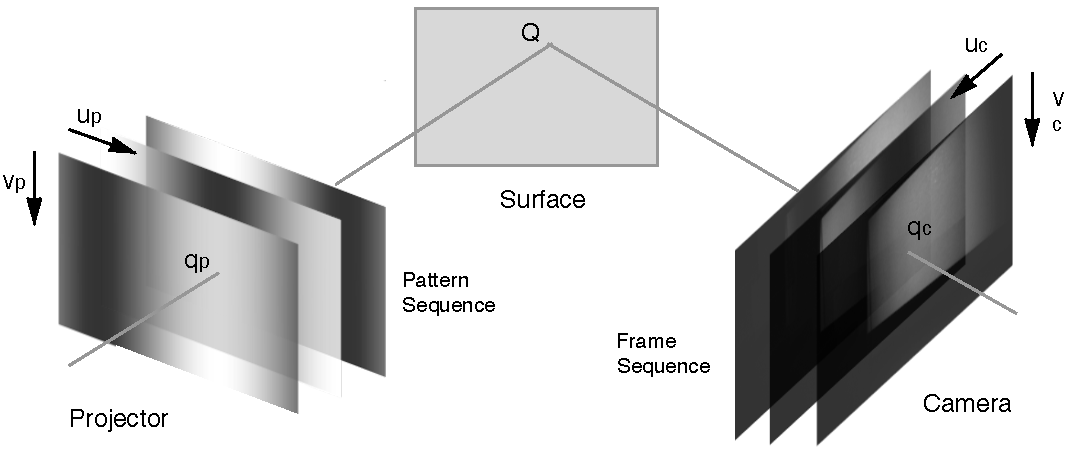
\includegraphics[width=0.80\linewidth]{figures/stl_principle}
  \end{figure}
}

\frame{
  \frametitle{Basic Ray Model}
  \begin{onlyenv}<1>
    \begin{figure}
      \centering
      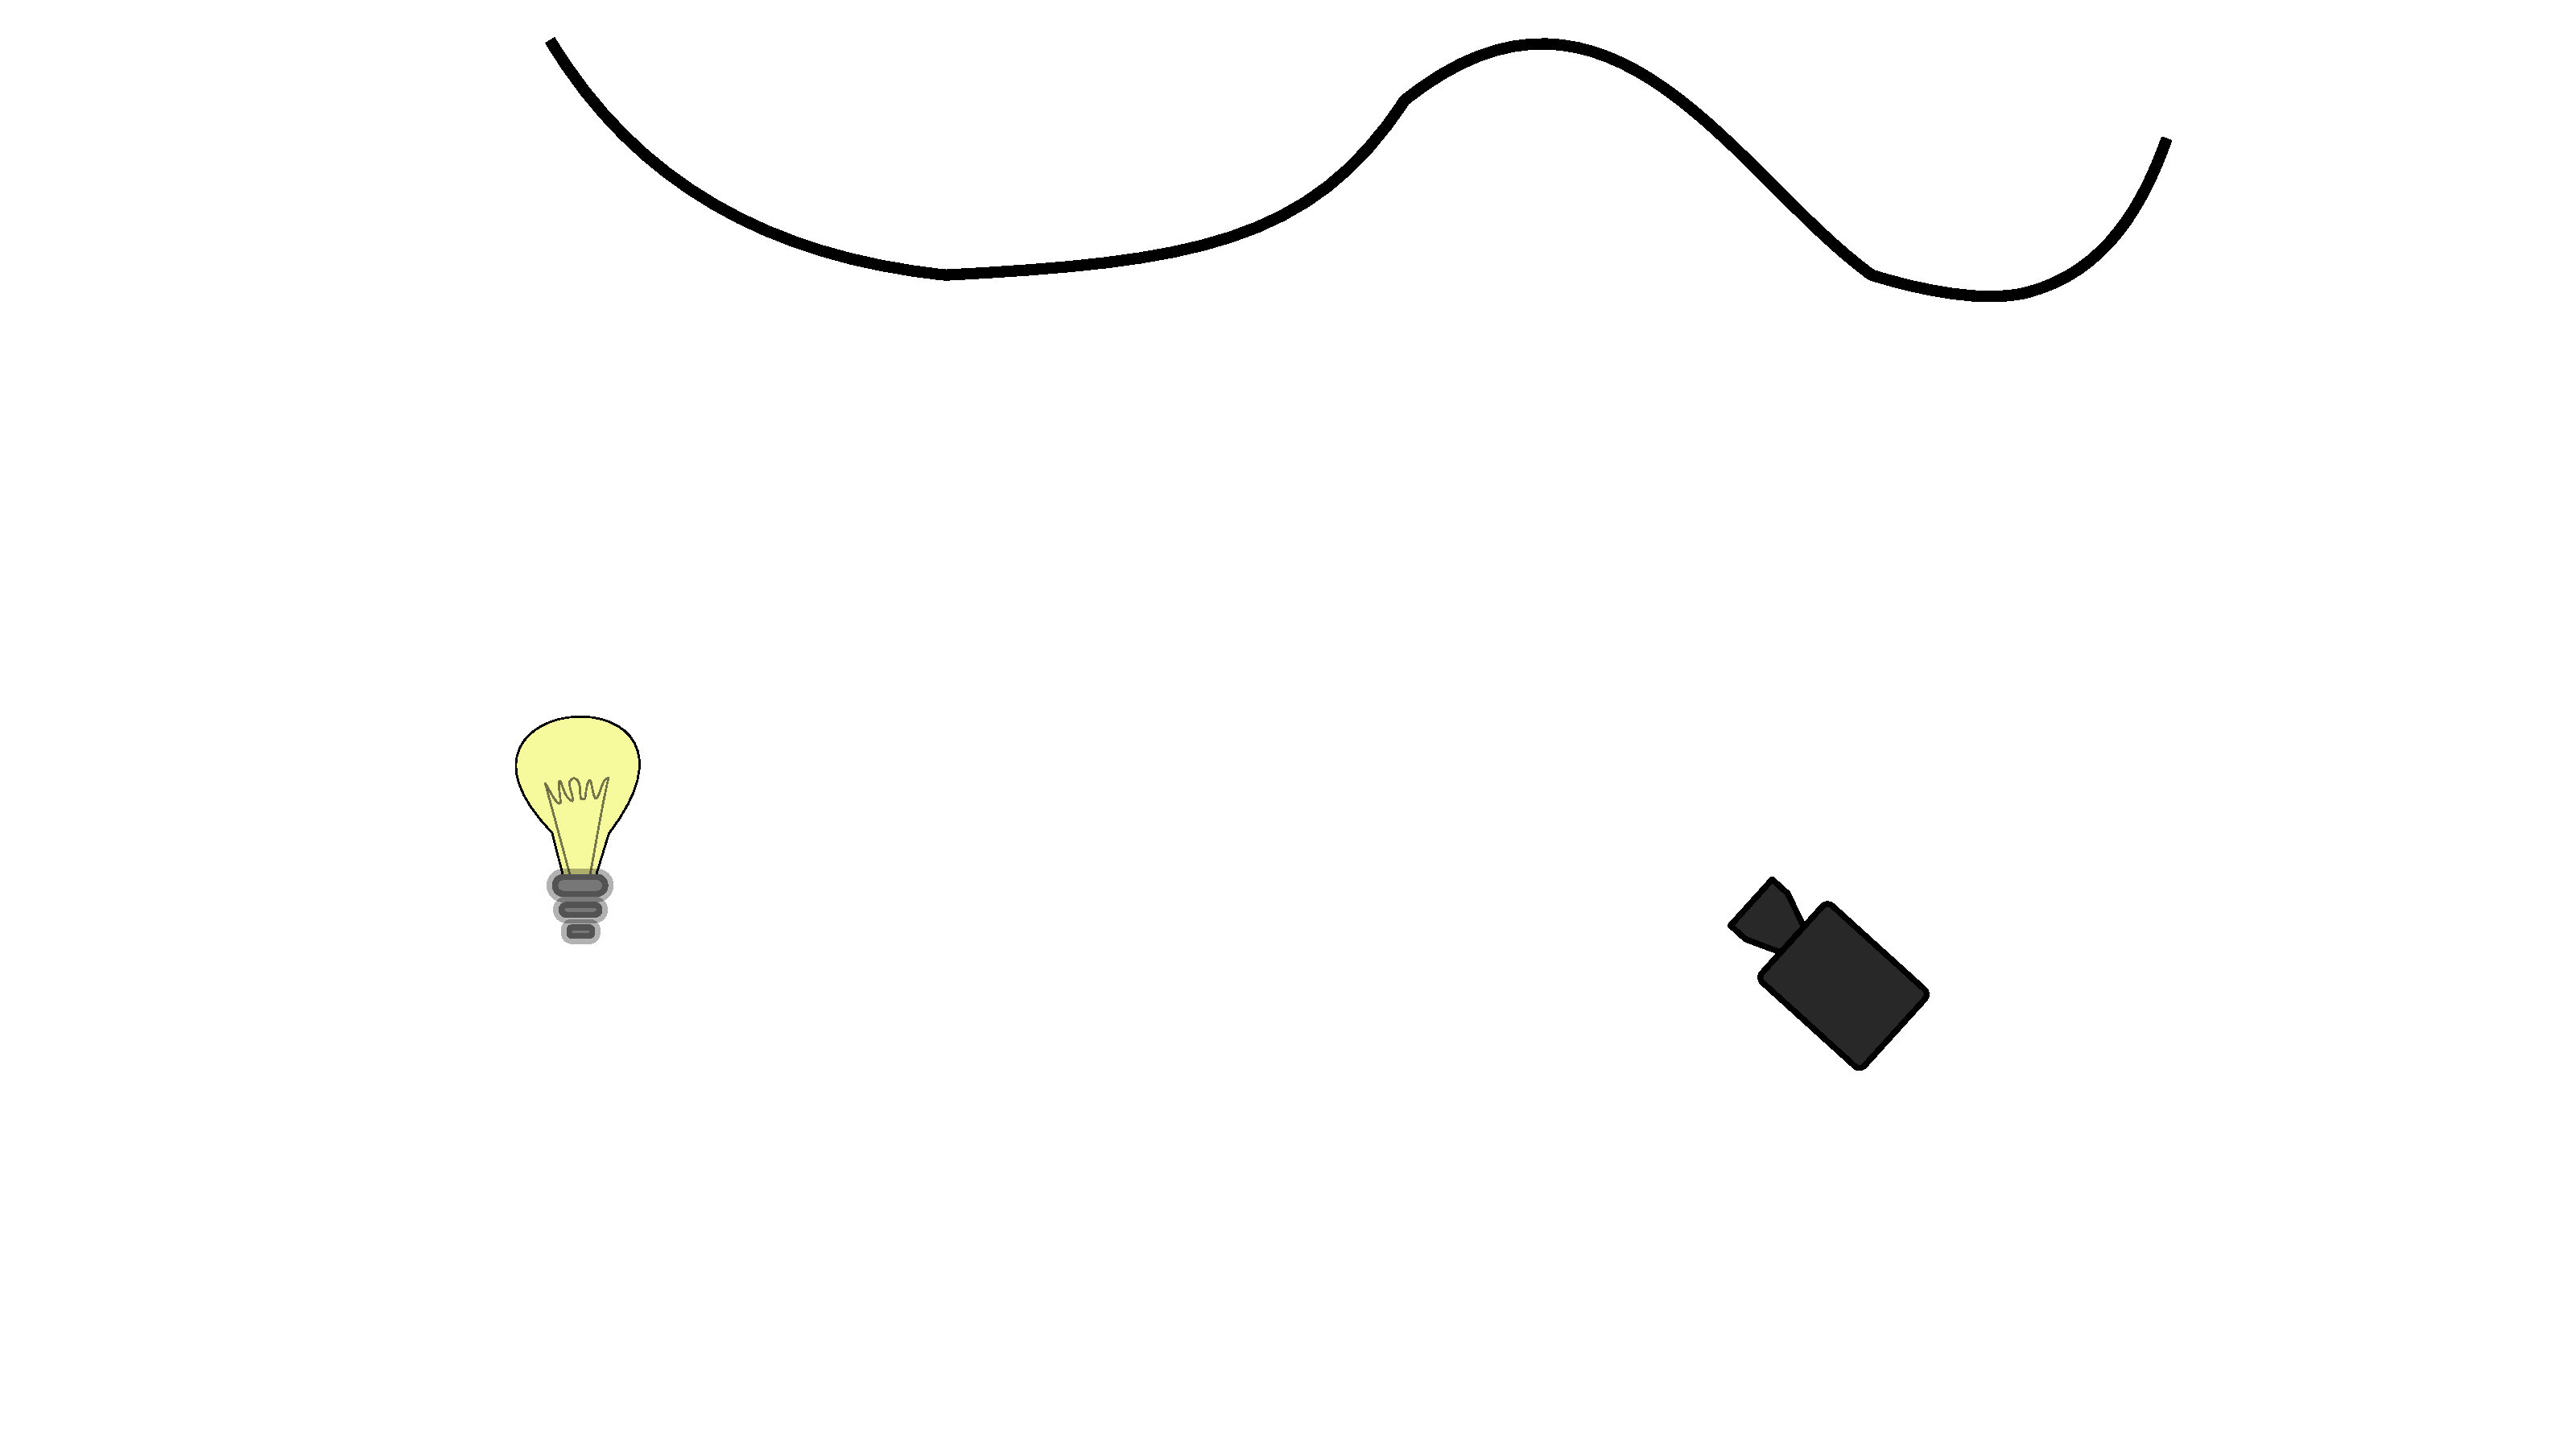
\includegraphics[width=0.8\linewidth]{figures/stl_none}
    \end{figure}
  \end{onlyenv}
  \begin{onlyenv}<2>
    \begin{figure}
      \centering
      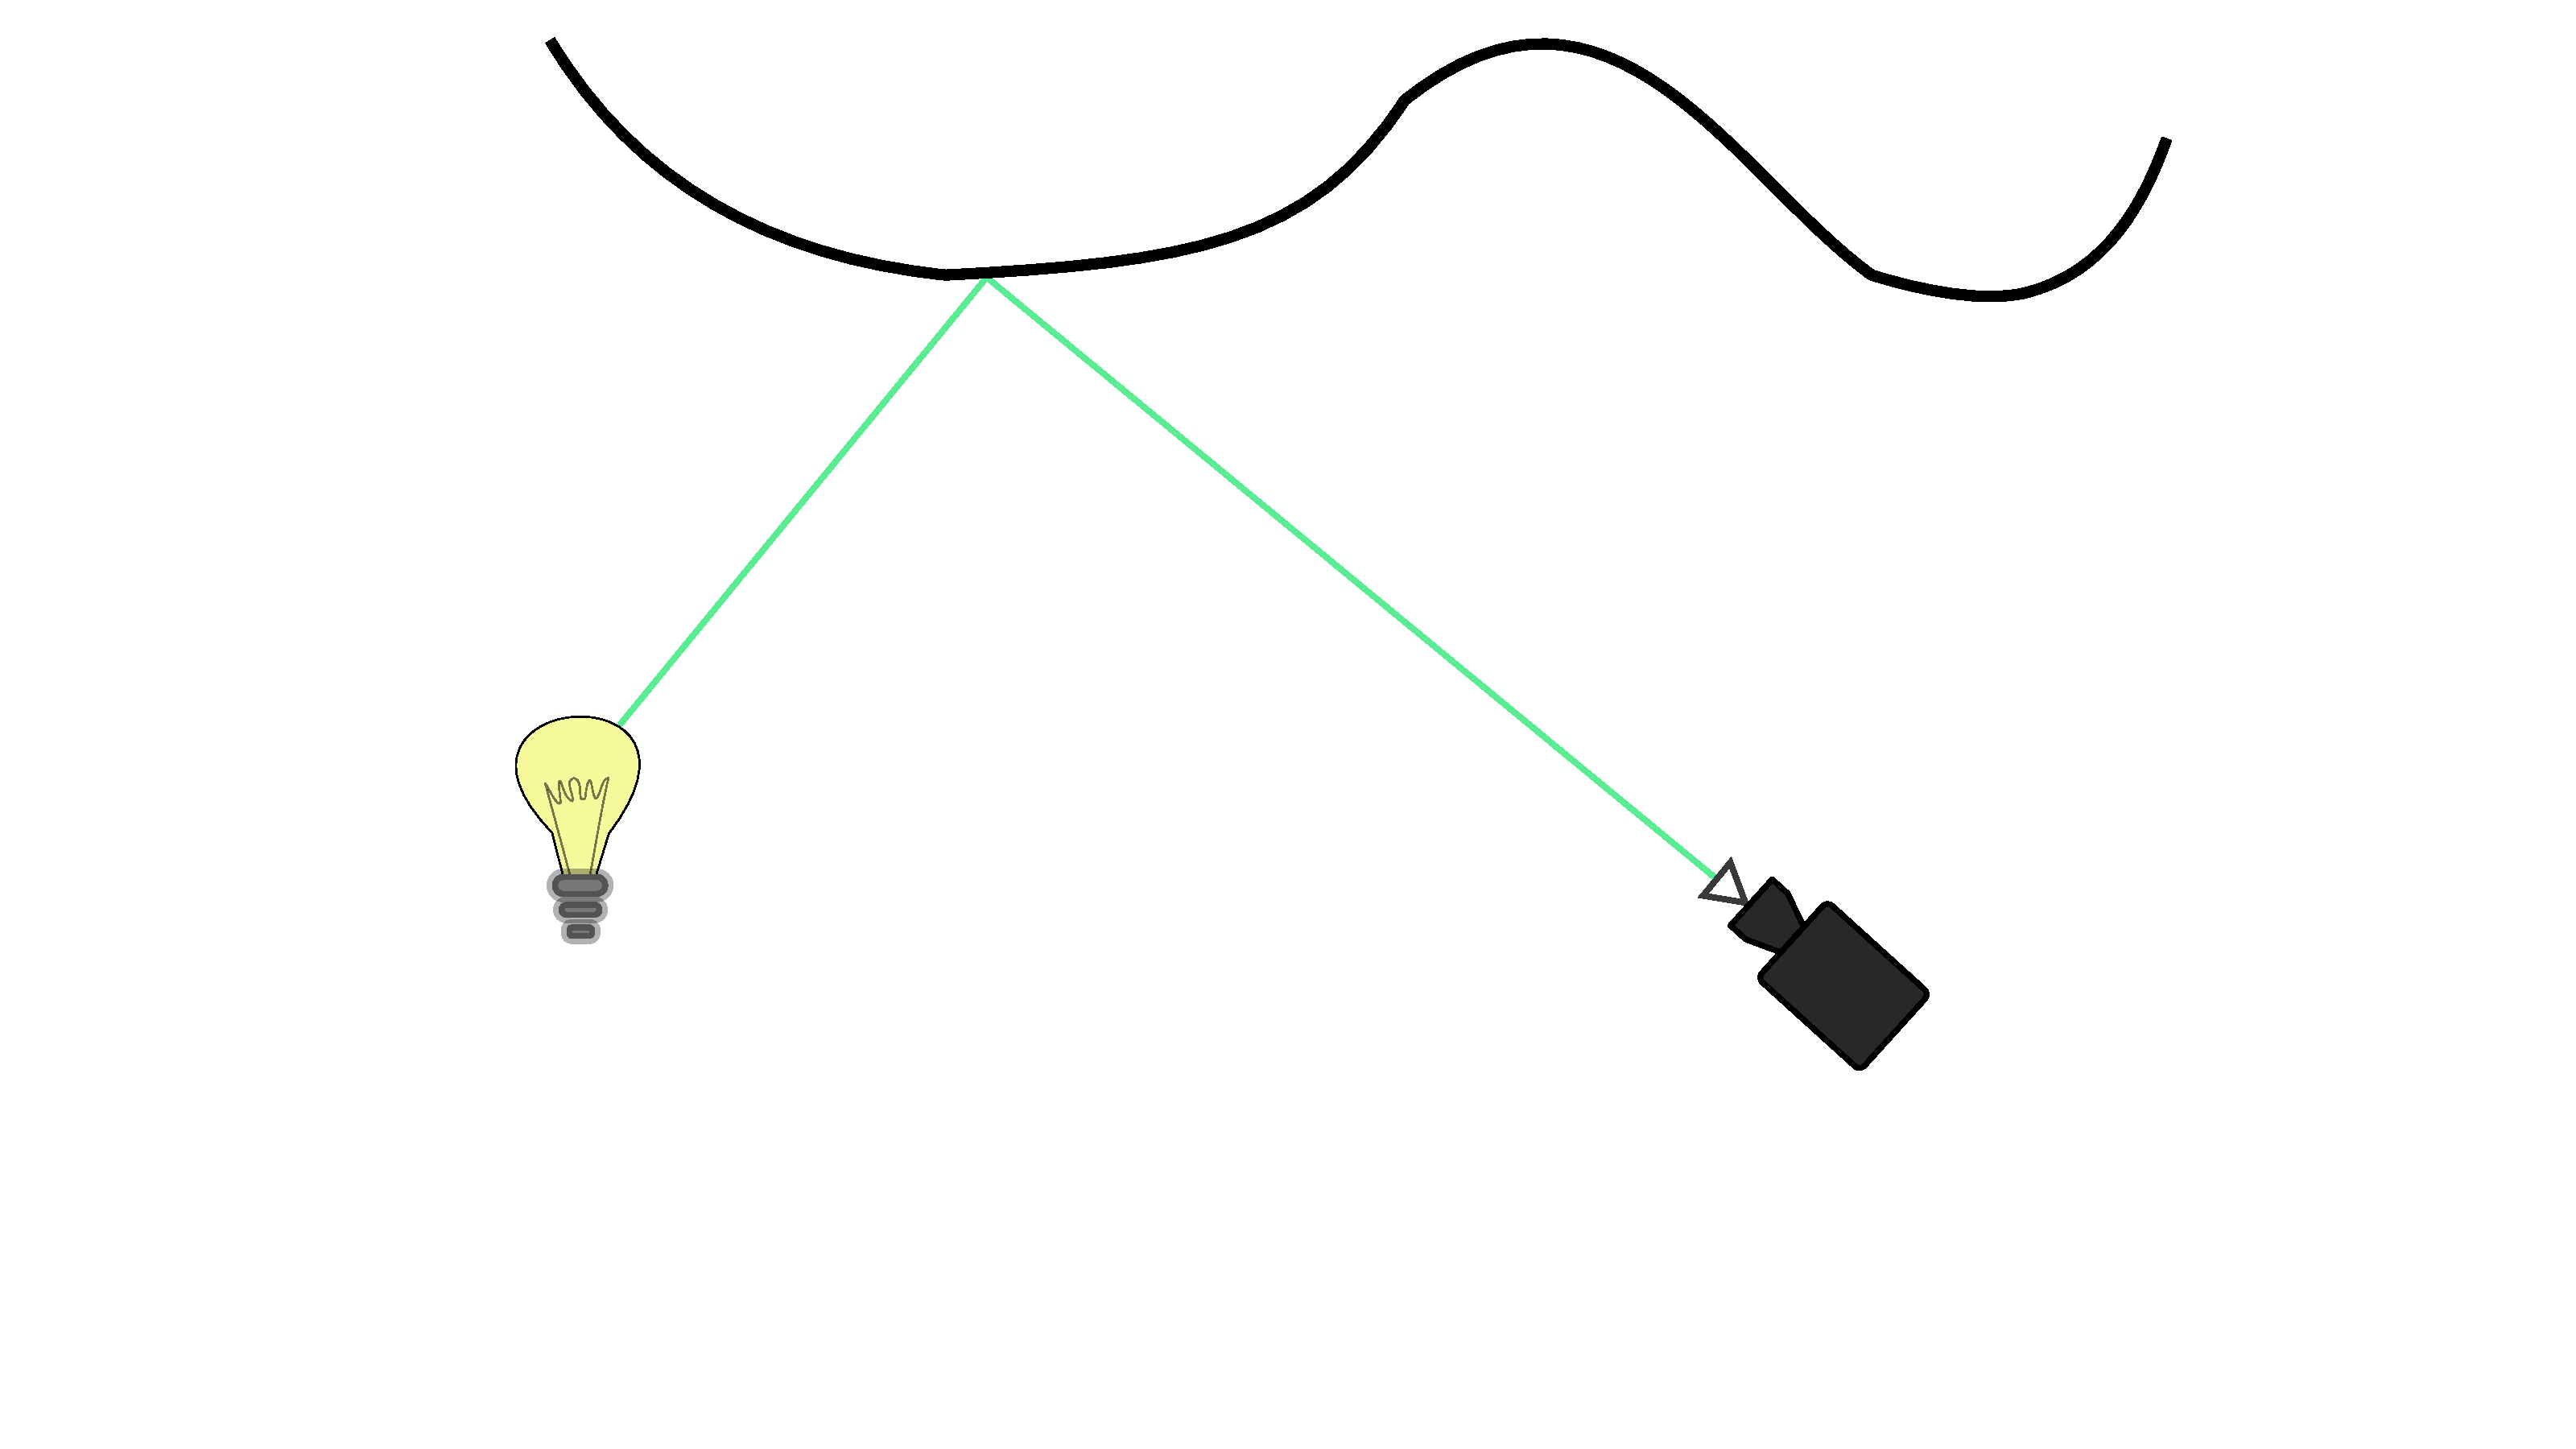
\includegraphics[width=0.8\linewidth]{figures/stl_direct}
    \end{figure}
  \end{onlyenv}
  \begin{onlyenv}<3>
    \begin{figure}
      \centering
      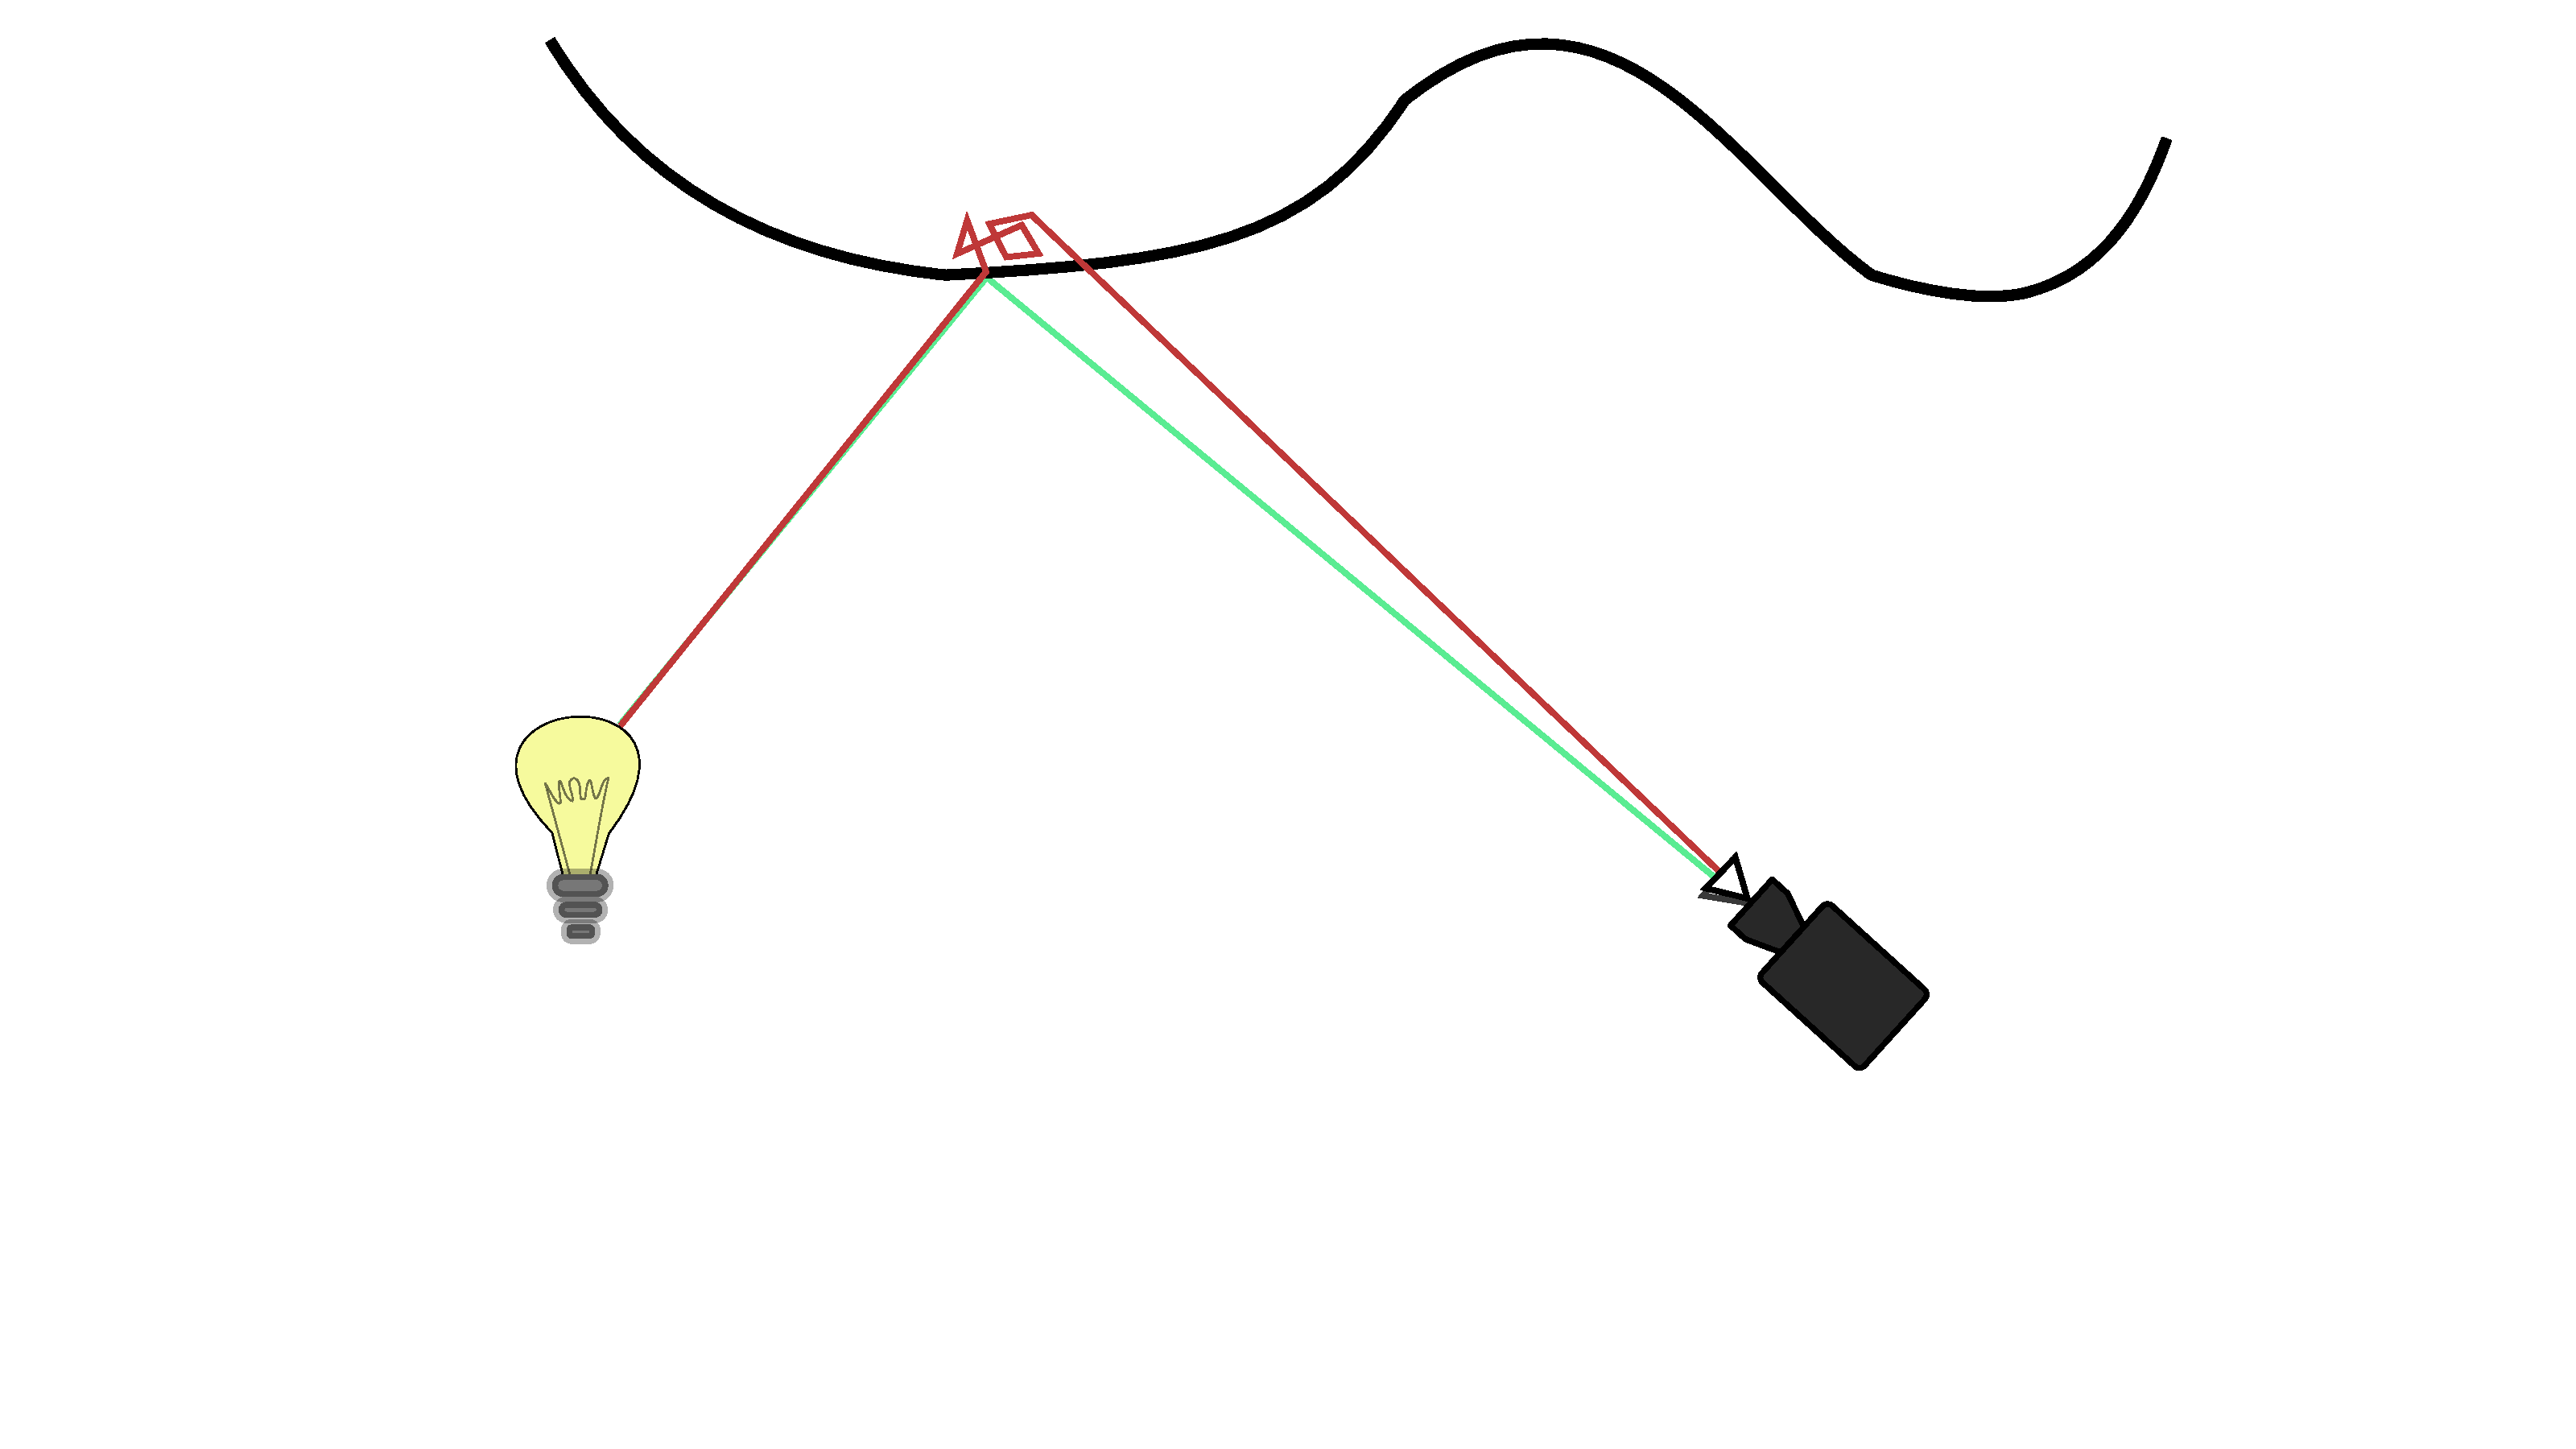
\includegraphics[width=0.8\linewidth]{figures/stl_all}
    \end{figure}
  \end{onlyenv}
}


\frame{
  \frametitle{Significance of Subsurface Scattering}
  \begin{figure}
    \centering
    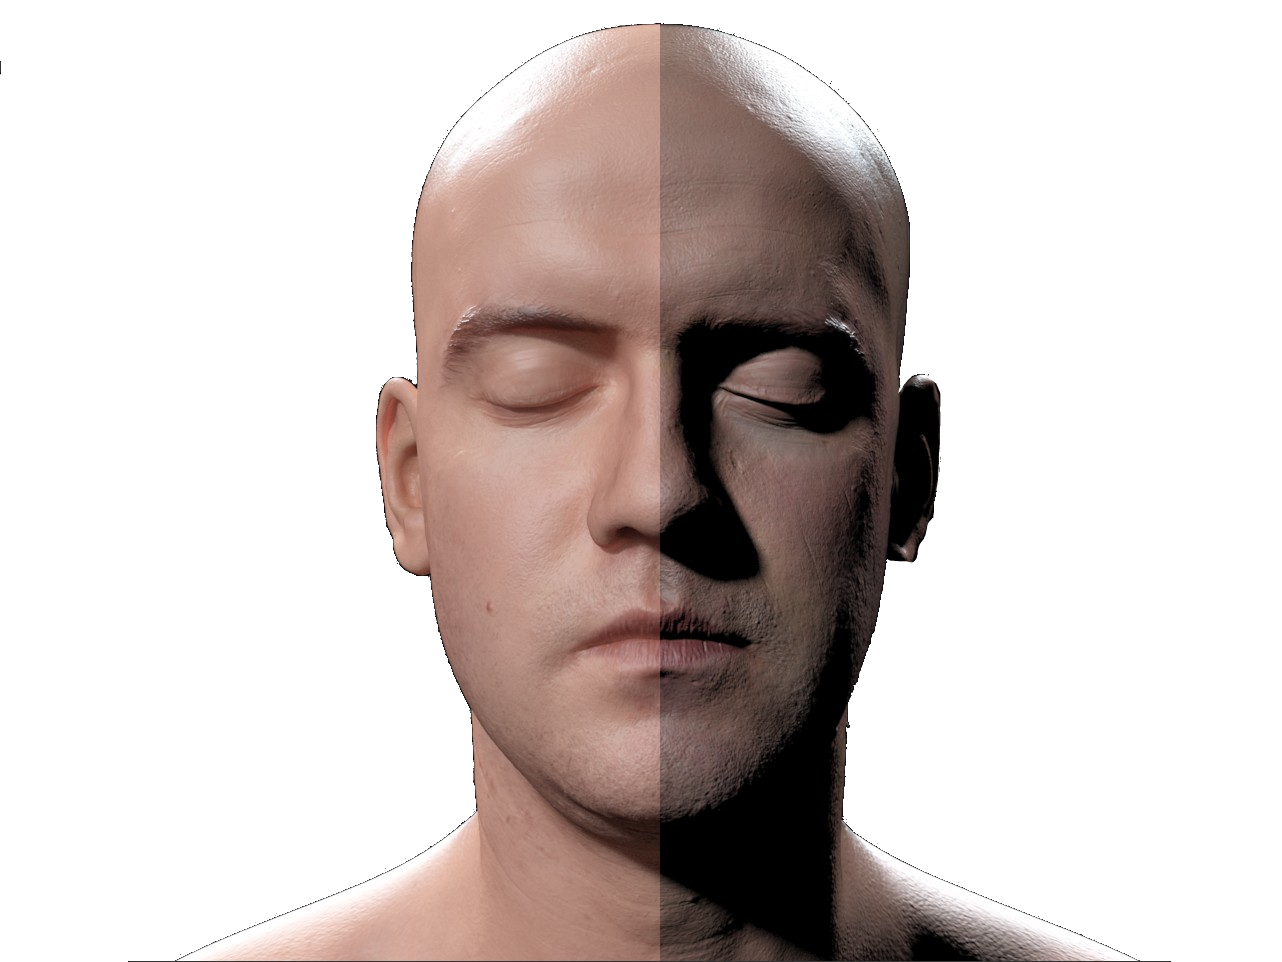
\includegraphics[height=0.8\textheight]{figures/humanss}
  \end{figure}
}

\frame{
  \frametitle{Materials and Structured Light Methods}
  \begin{minipage}[t]{0.48\linewidth}
    \captionsetup[subfloat]{position=above, labelformat=empty}
    \begin{figure}
      \subfloat[Skin]{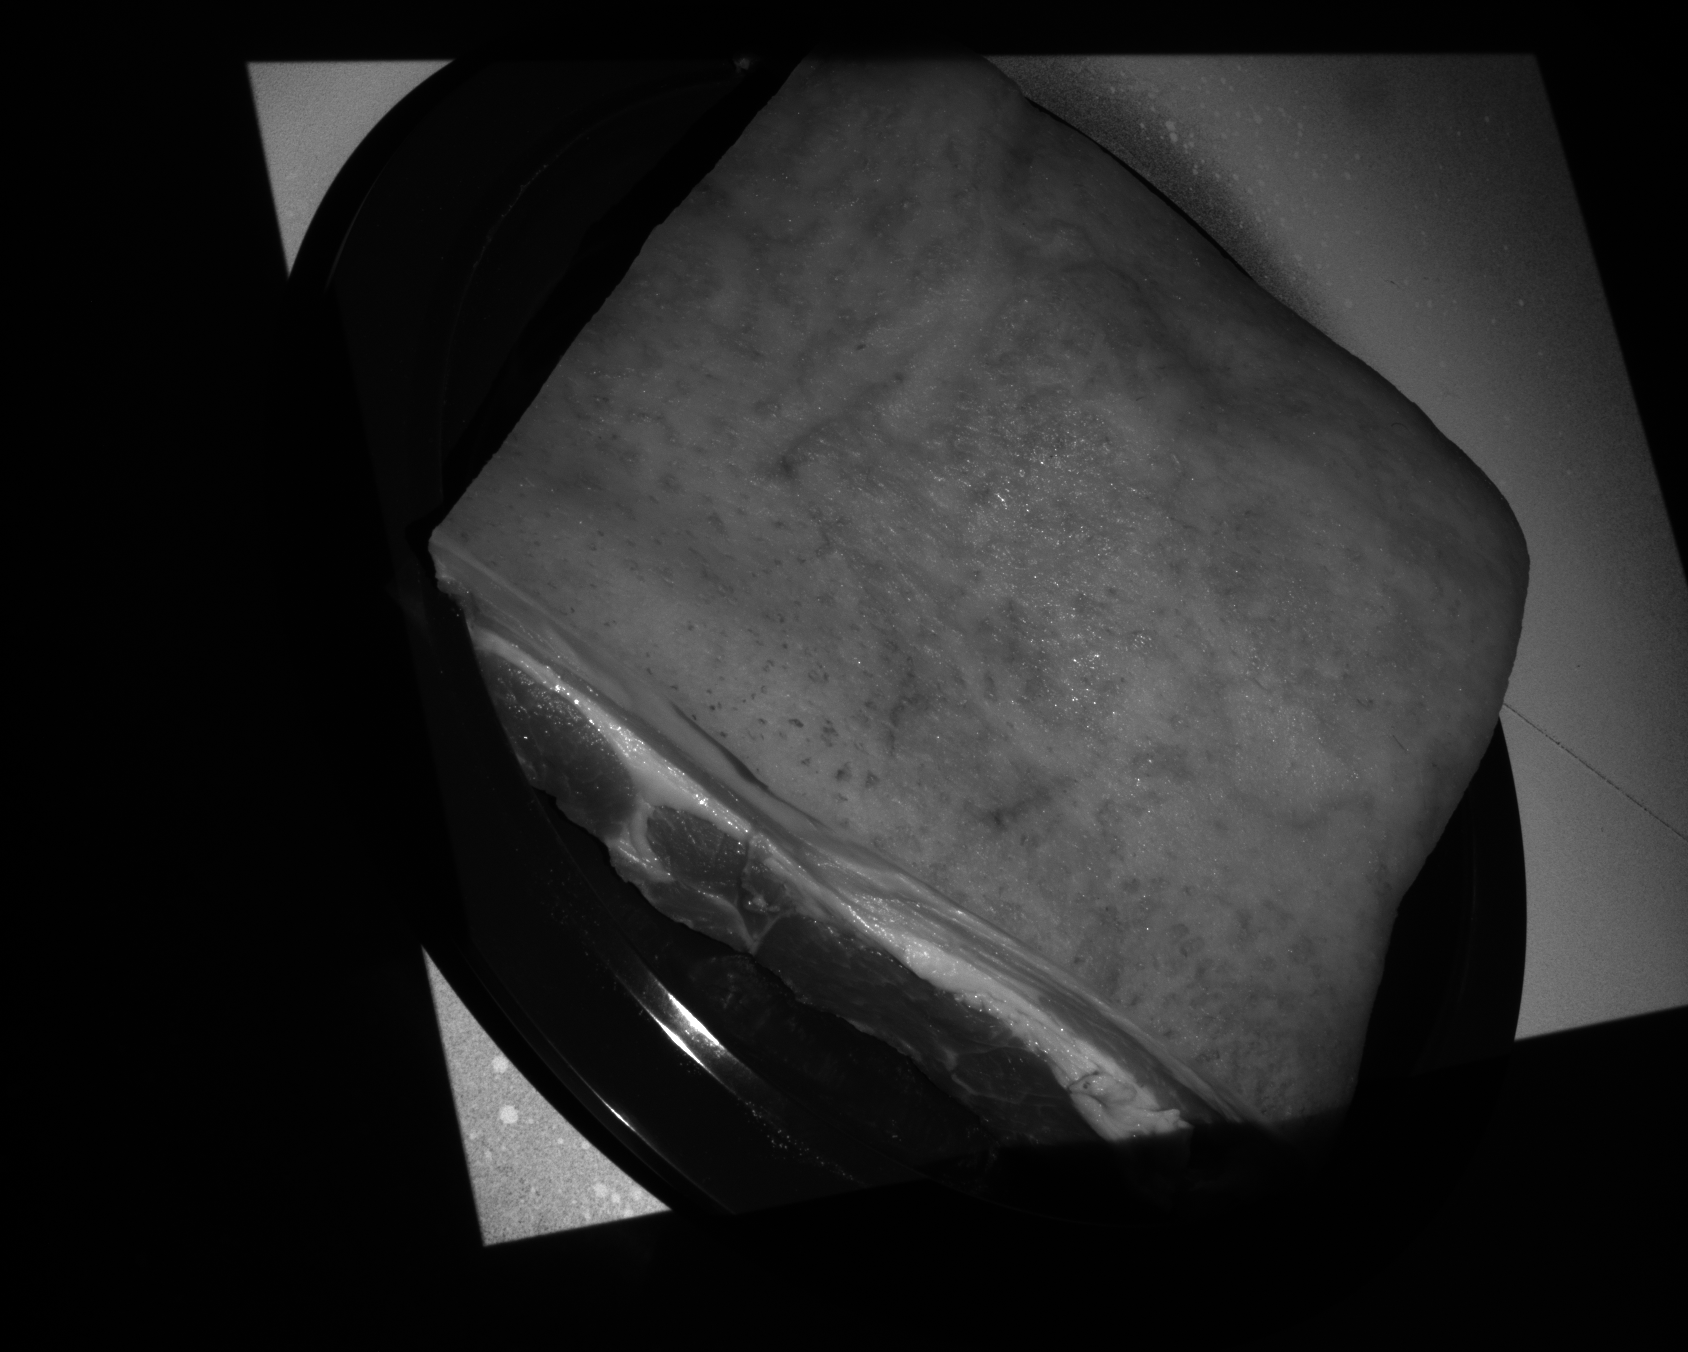
\includegraphics[width=0.49\linewidth]{figures/skin}}\hfill
      \subfloat[Fat]{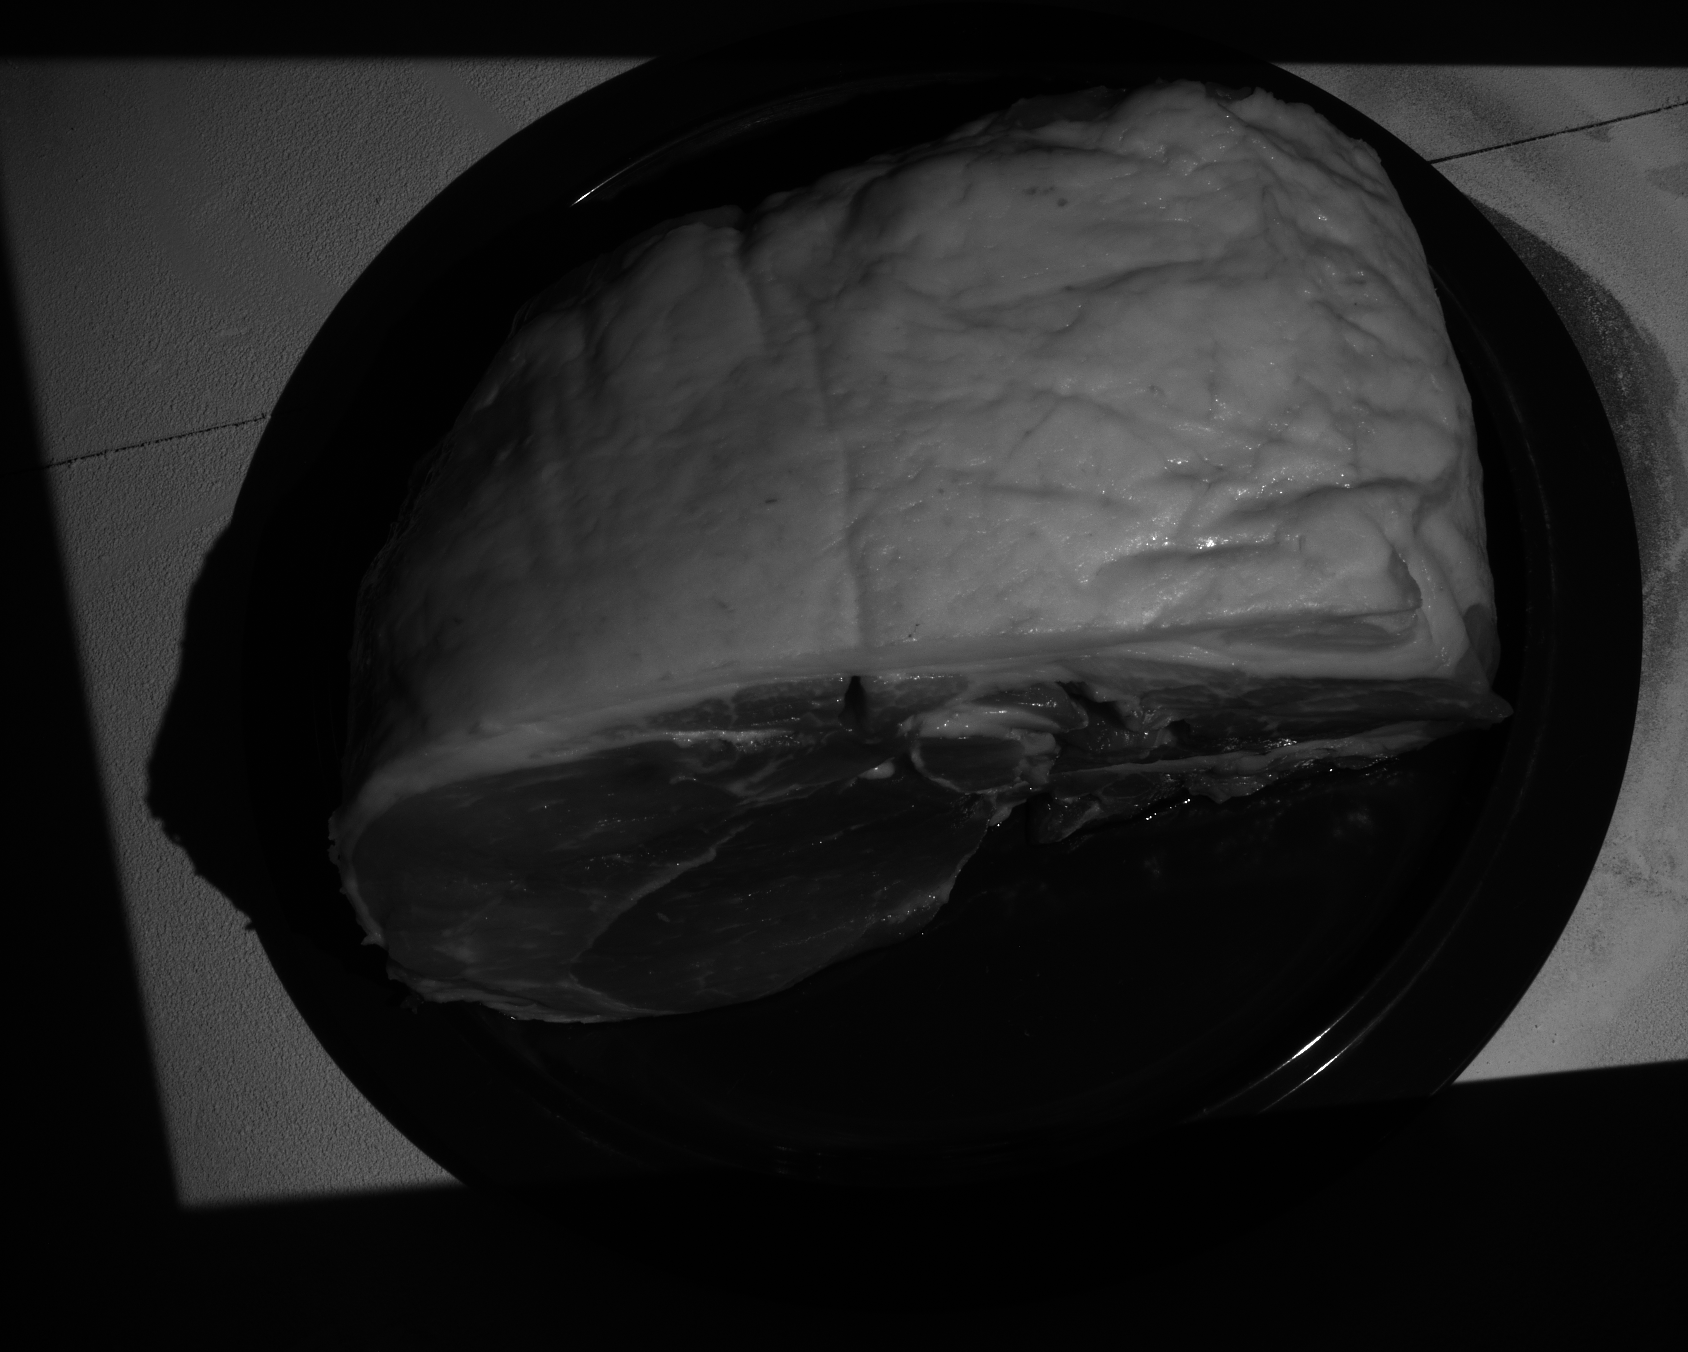
\includegraphics[width=0.49\linewidth]{figures/fat}}
    \end{figure}
    \captionsetup[subfloat]{position=below, labelformat=empty}
    \vspace{-1cm}
    \begin{figure}
      \subfloat[Meat]{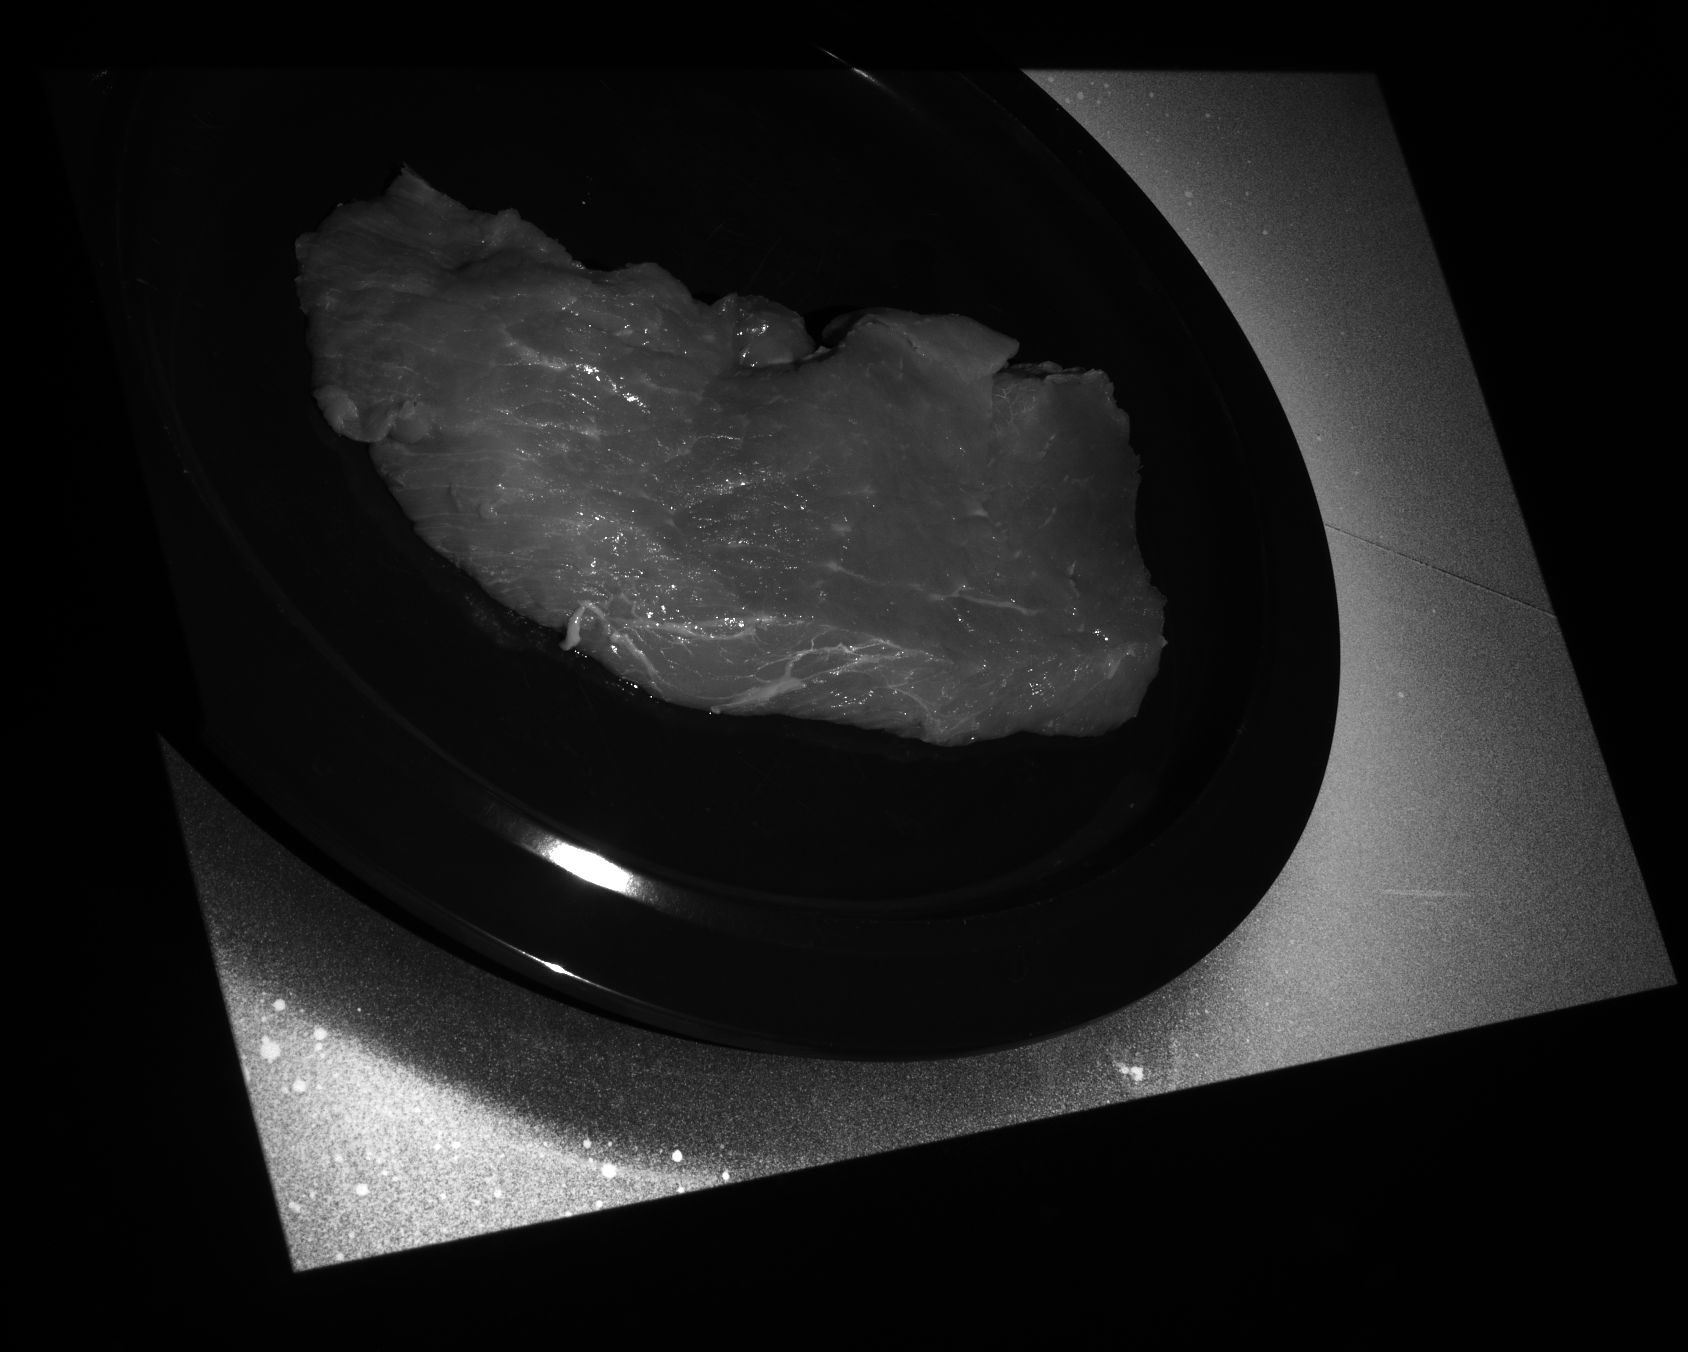
\includegraphics[width=0.49\linewidth]{figures/muscle}}
    \end{figure}
  \end{minipage}\hfill
  \begin{minipage}[t]{0.48\linewidth}
    \captionsetup[subfloat]{position=above, labelformat=empty}
    \begin{figure}
      \subfloat[Gray Codes~\cite{posdamer1982surface}]{
\includegraphics[width=0.49\linewidth]{figures/pattern}}\hfill
      \subfloat[Phase Shifting~\cite{Huntley1993a}]{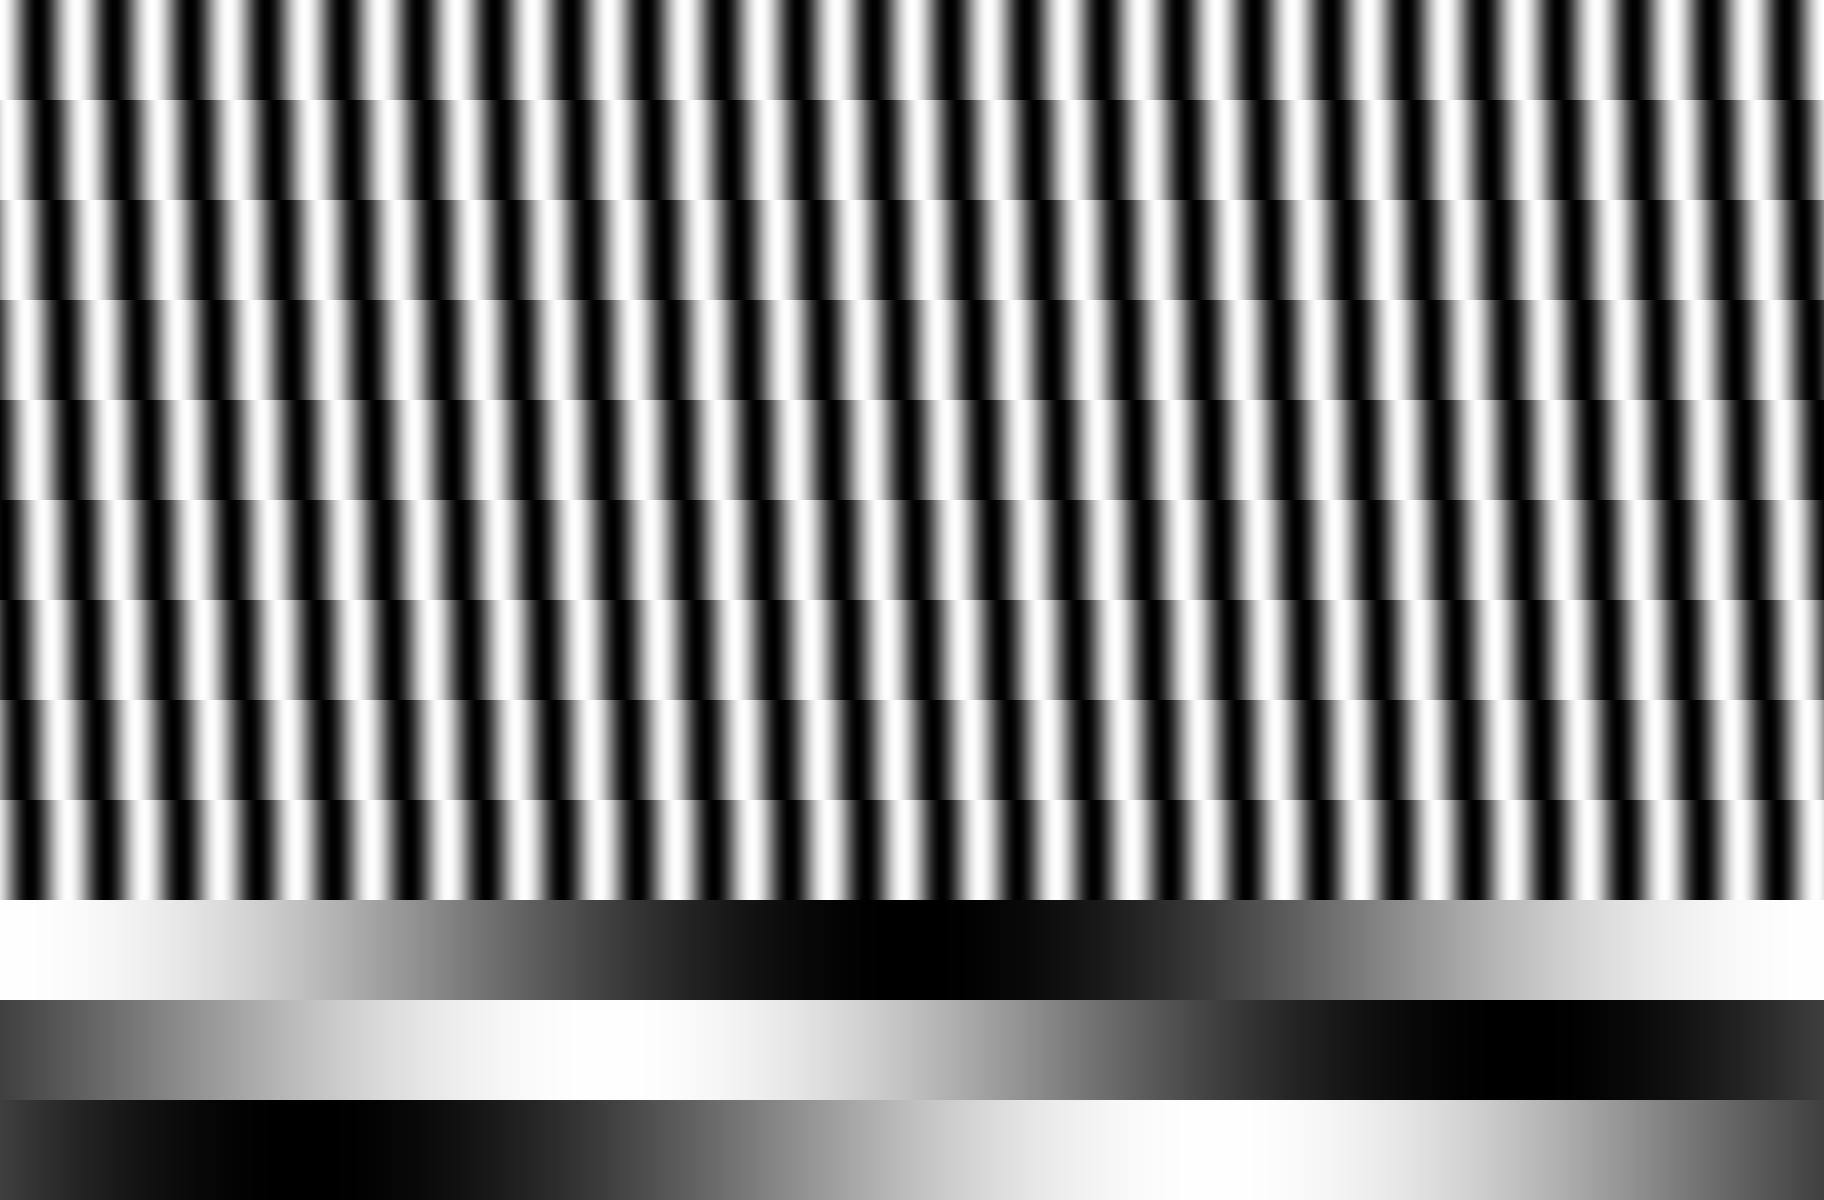
\includegraphics[width=0.49\linewidth]{figures/patterns_nstep}}
    \end{figure}
    \captionsetup[subfloat]{position=below, labelformat=empty}
    \vspace{-1cm}
    \begin{figure}
      \subfloat[Modulated Phase Shifting~\cite{chen2008modulated}]{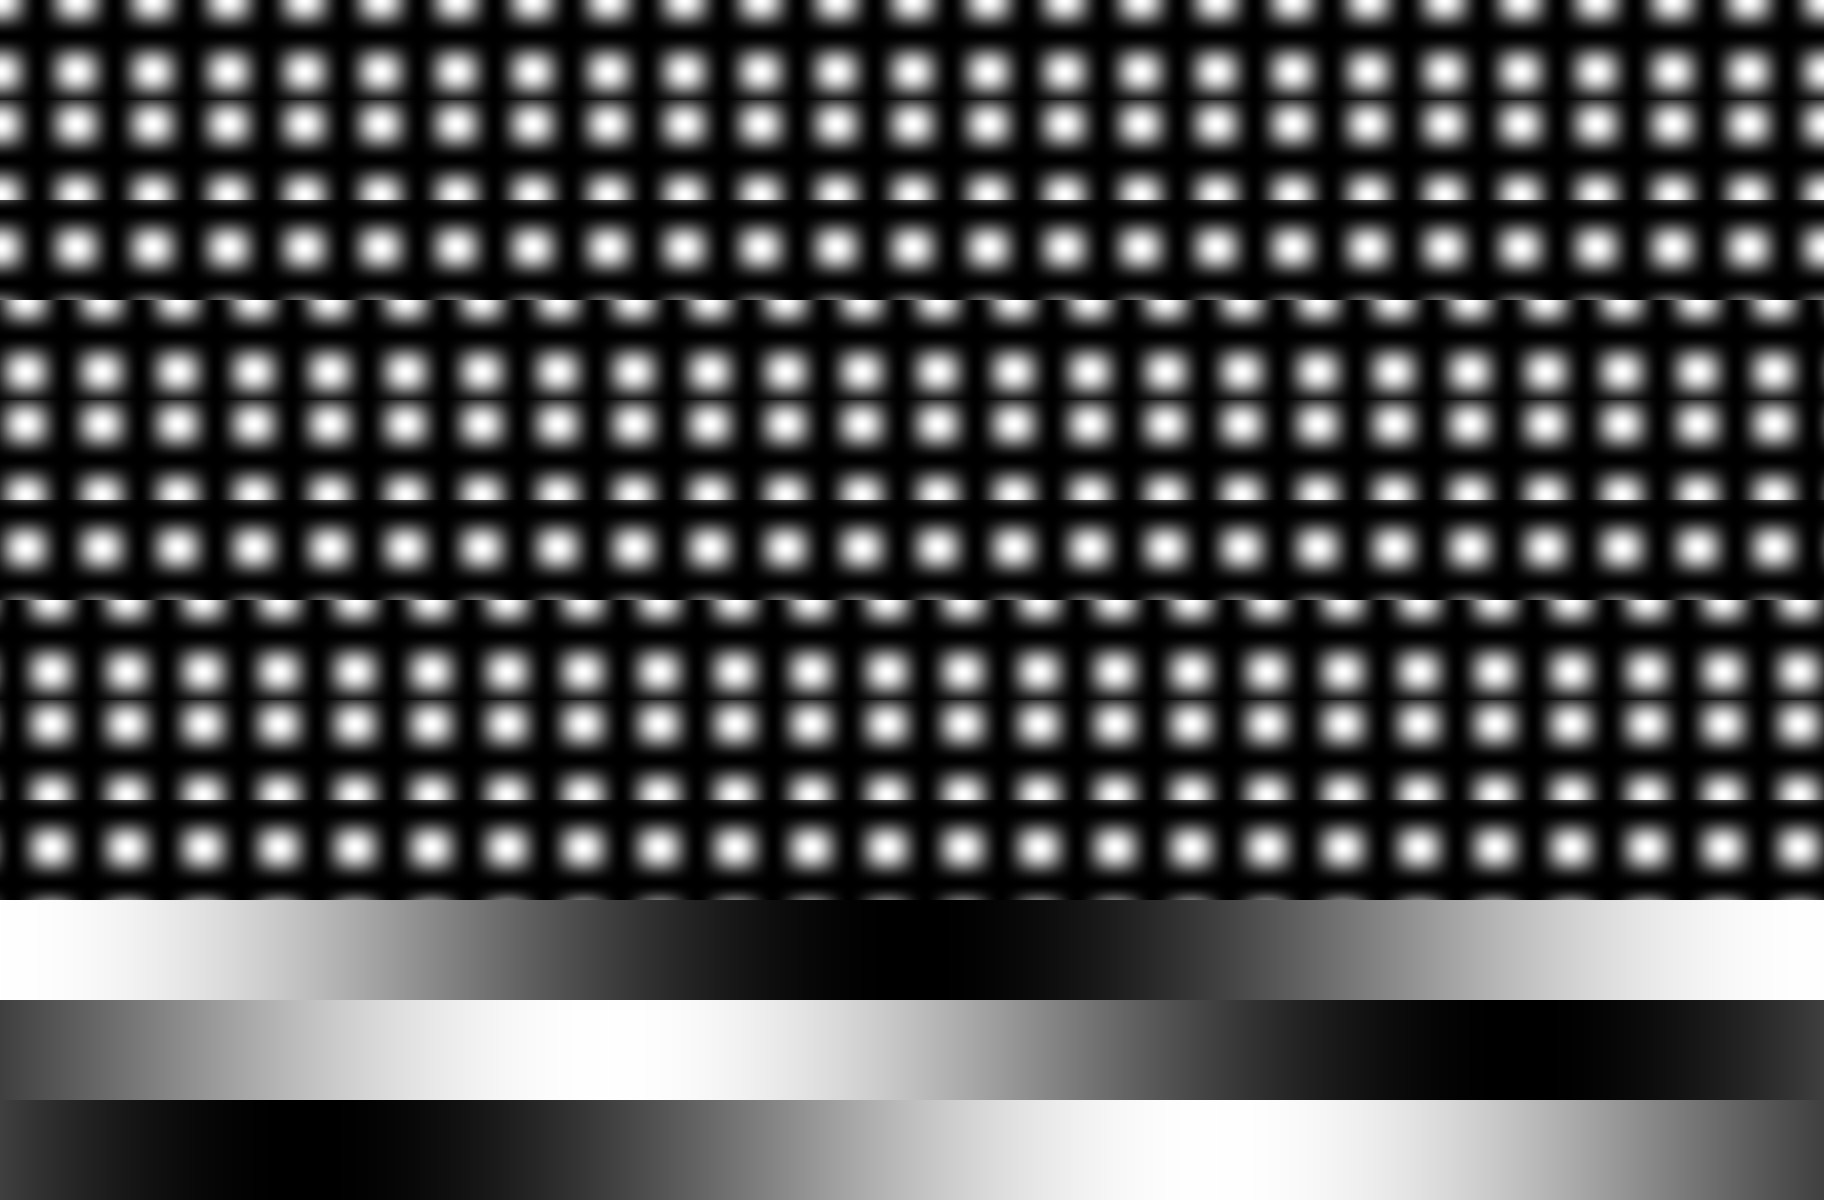
\includegraphics[width=0.49\linewidth]{figures/patterns_modulated}}\hfill
      \subfloat[Micro Phase Shifting~\cite{gupta2012micro}]{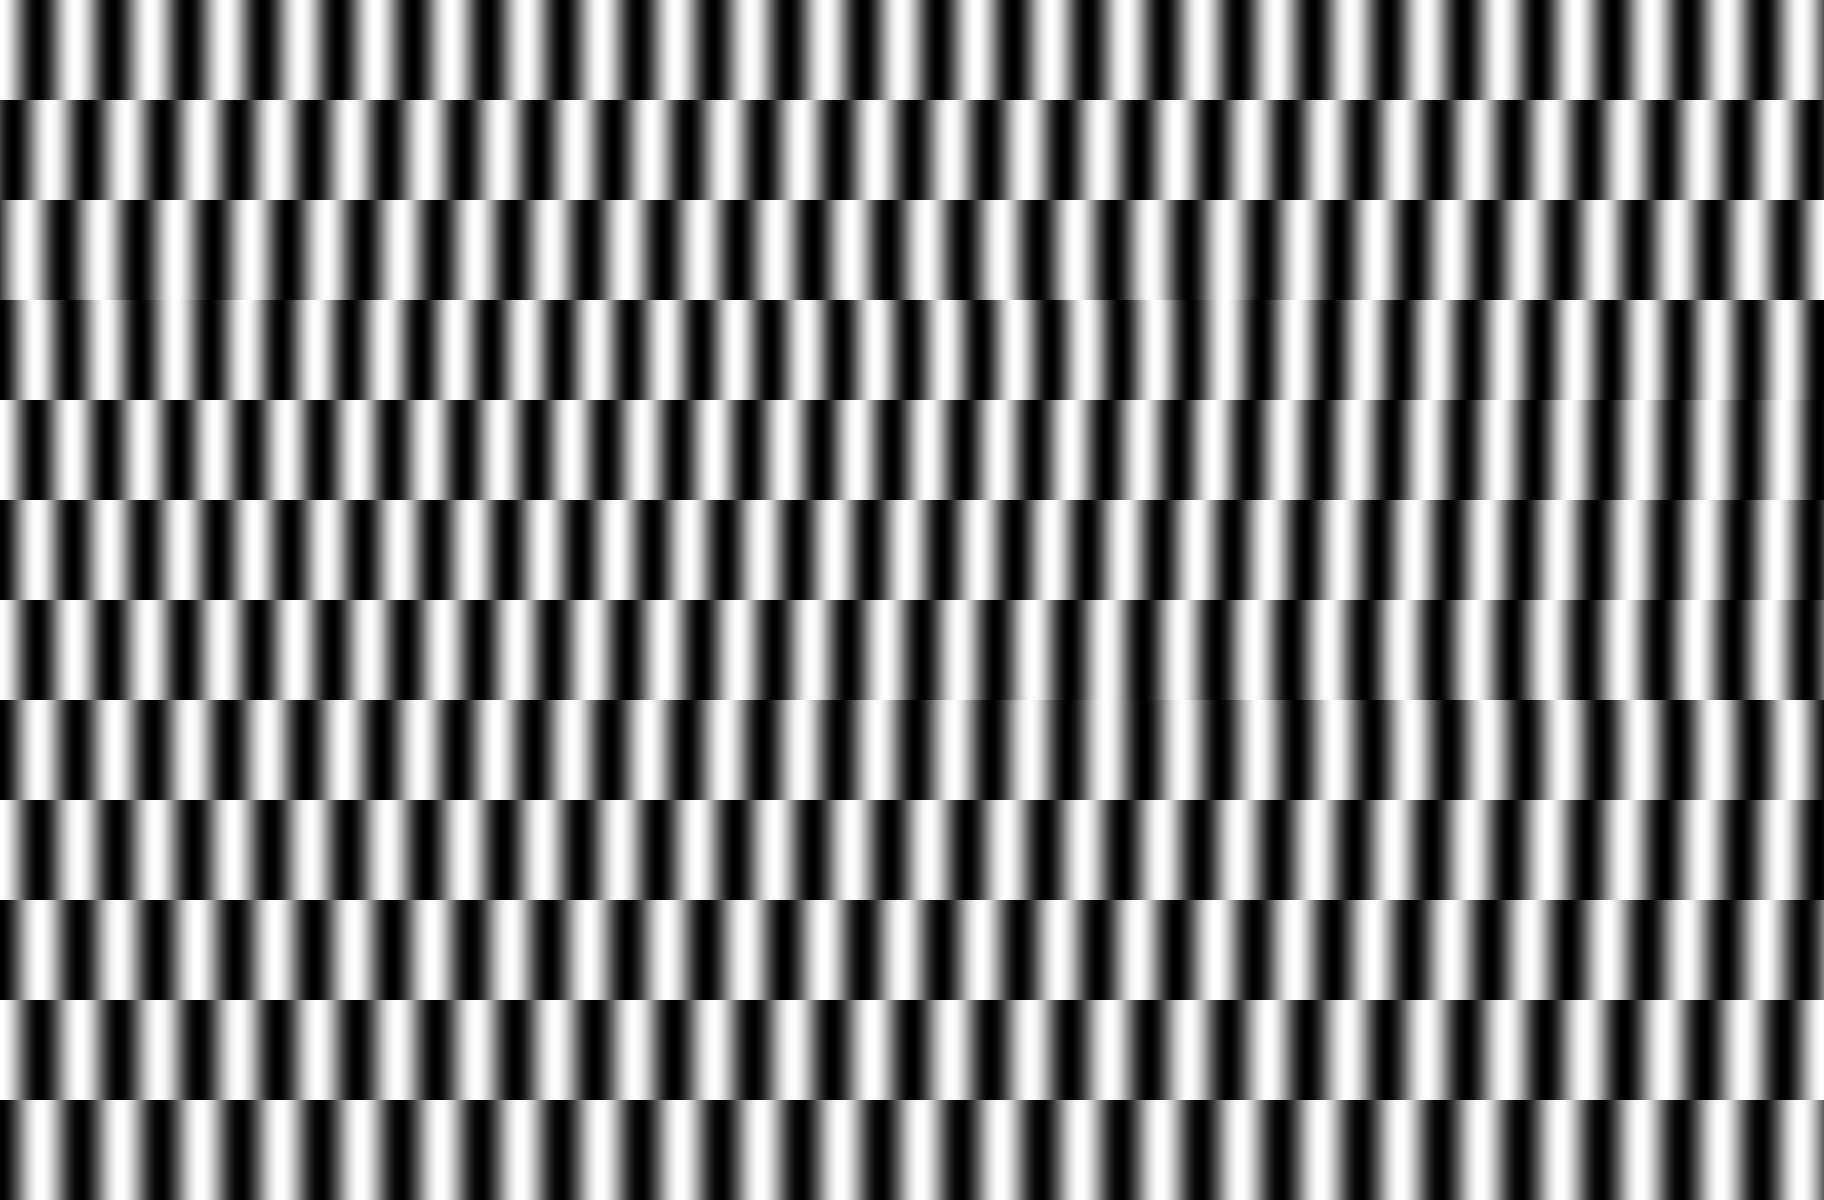
\includegraphics[width=0.49\linewidth]{figures/patterns_micro}}
    \end{figure}
  \end{minipage}
}

\frame{
  \frametitle{Reference Acquisition using Chalk Coating}
  \begin{figure}
    \centering
    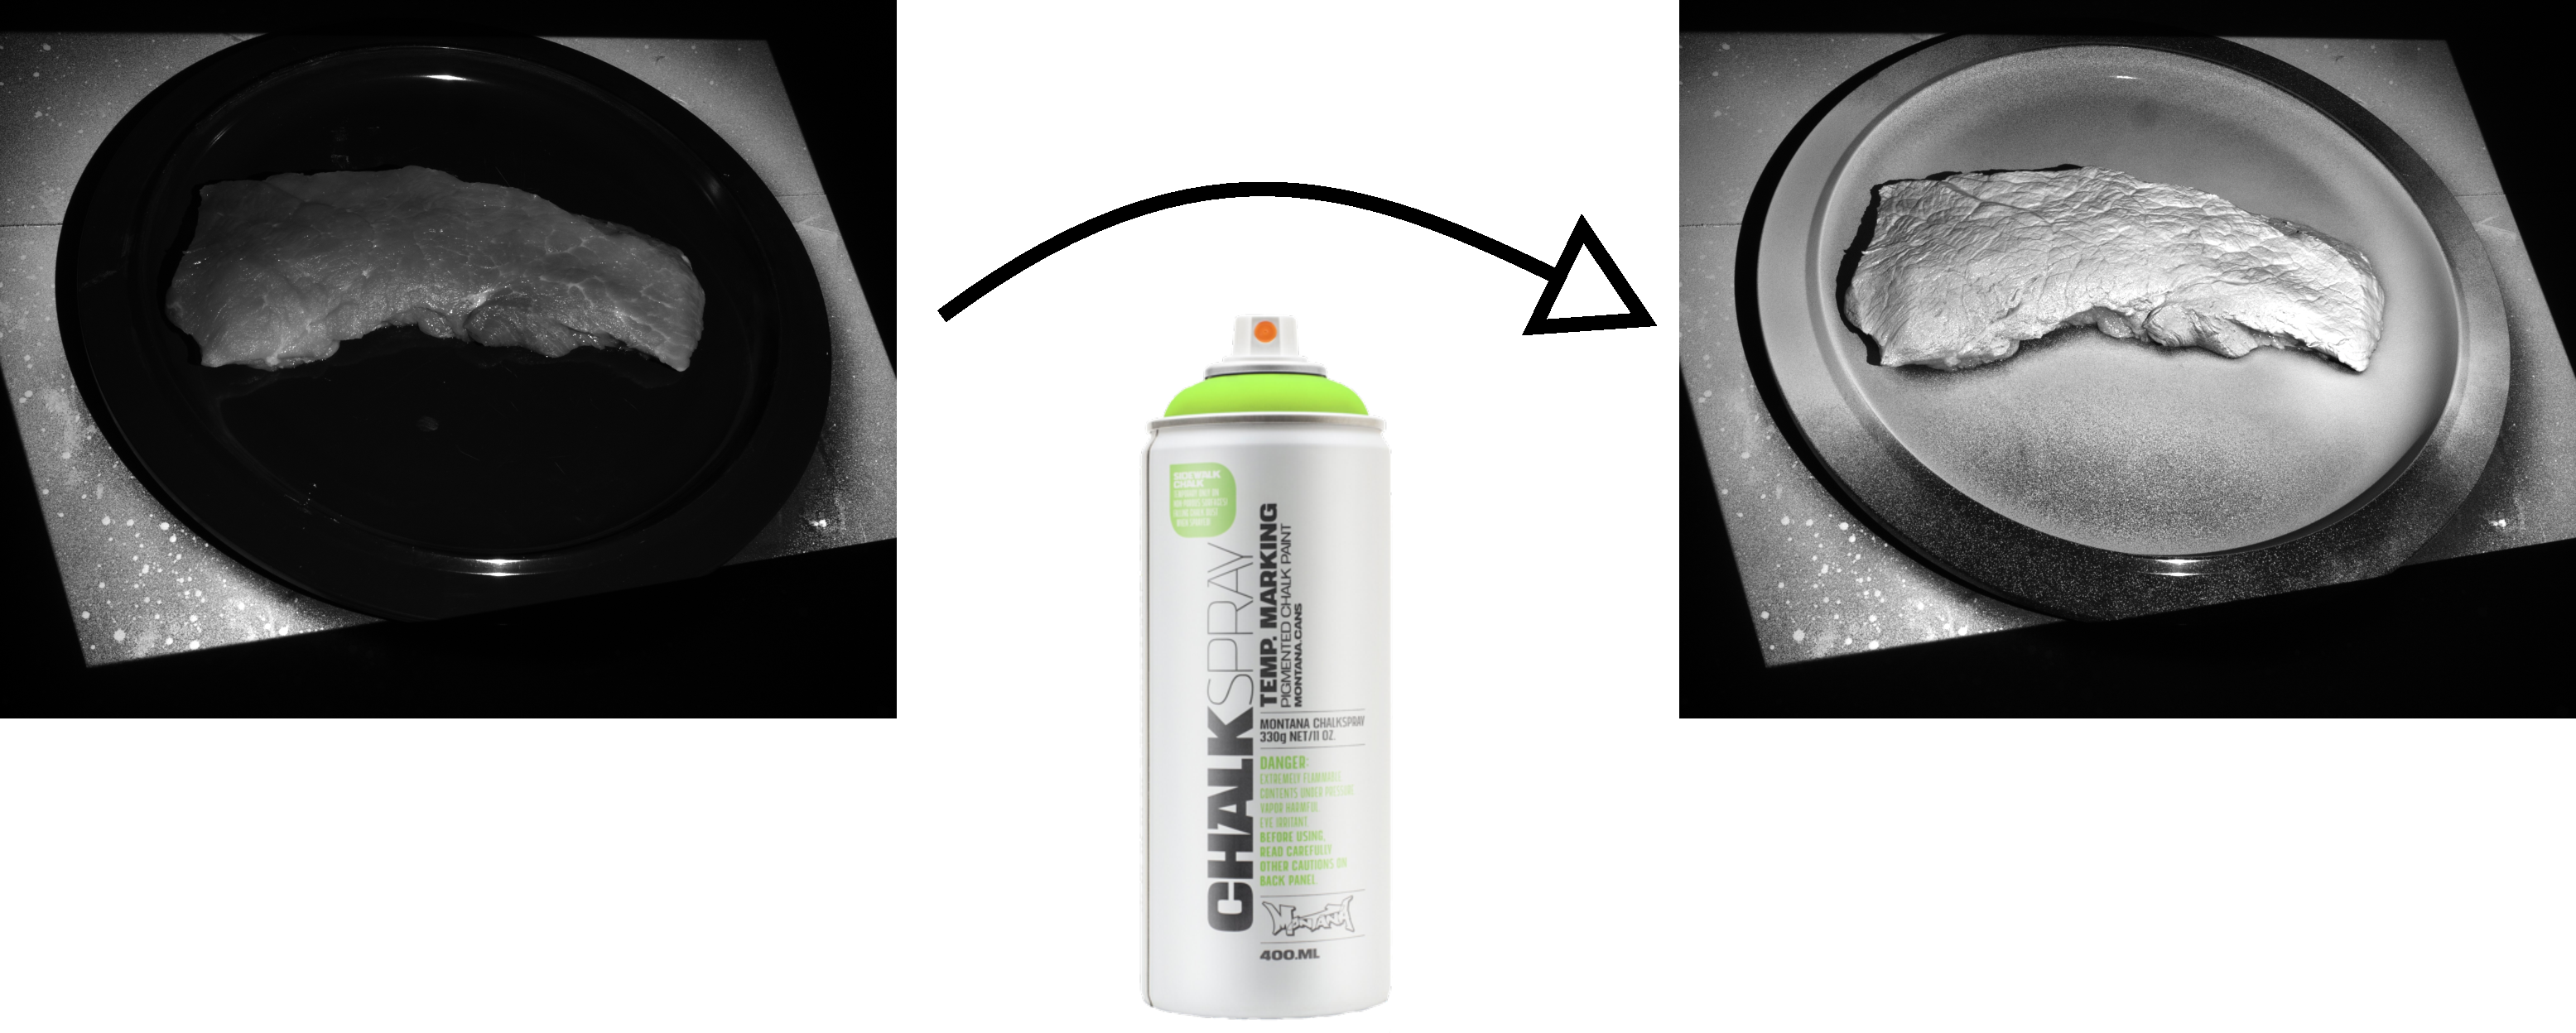
\includegraphics[width=0.95\linewidth]{figures/chalk_reference}
  \end{figure}
}

\frame{
  \frametitle{Boxplot of Reconstruction Error, Skin}
  \begin{figure}
    \centering
    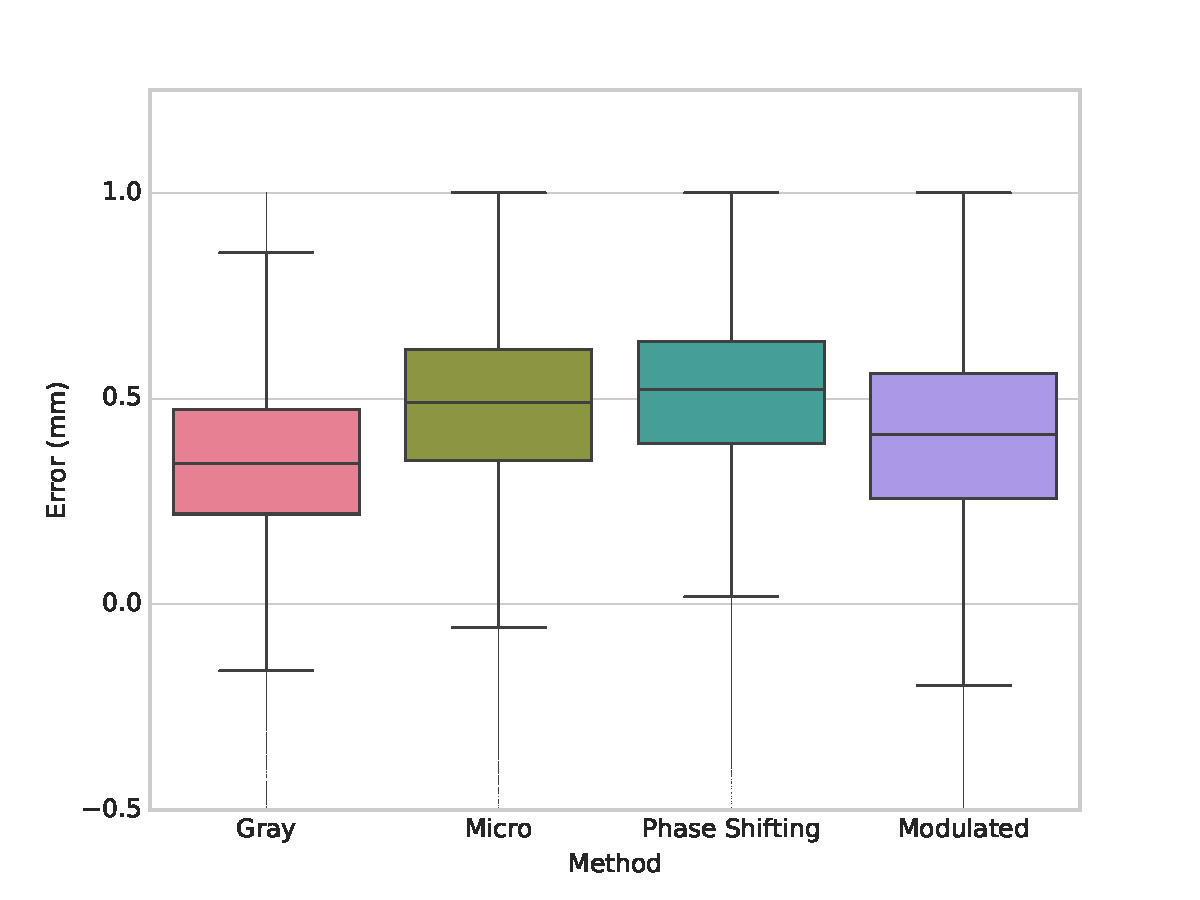
\includegraphics[height=0.85\textheight]{figures/boxplot_error}
  \end{figure}
}

\frame{
  \frametitle{Model}
  \begin{minipage}{0.48\textwidth}
    \begin{figure}
      \centering
      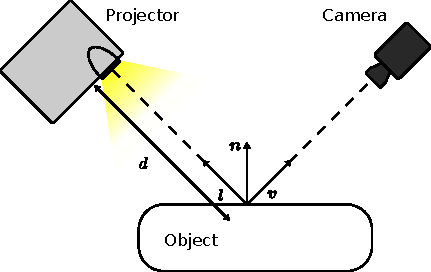
\includegraphics[height=0.65\textheight]{figures/camproj}
    \end{figure}
  \end{minipage}
  \hfill
  \begin{minipage}{0.48\textwidth}
    \begin{align}
      y = \begin{bmatrix} 1 & \mathbf{n} \cdot \mathbf{v} & \mathbf{n} \cdot \mathbf{l} & d \end{bmatrix}
      \begin{bmatrix}
        \beta_0\\
        \beta_1\\
        \beta_2\\
        \beta_3
      \end{bmatrix}
    \end{align}
  \end{minipage}
}

\frame{
\frametitle{Results}
  \begin{onlyenv}<1>
    \begin{table}
    \caption{Muscle model estimate and regression quality}
      \label{tab:parameters_muscle}
      %\centering

      \begin{tabular}{c|c c c c c c c c}
          & $\beta_0$ & $\beta_1$ & $\beta_2$ & $\beta_3$ & RMS$_\text{raw}$ & RMS$_\text{cor}$ & $R^2$ & $P$ \\\hline
          Gray & 0.13 & 0.15 & -0.026 & \num{2.3e-4} &  \textbf{0.42} & 0.27 & 0.0082 & 0 \\
          Phase Shifting & 0.25 & 0.47 & -0.18 & \num{-2.5e-5} & 0.5 & \textbf{0.21} & 0.06 & 0\\
          Micro PS & 0.21 & 0.36 & -0.12 & \num{-4.1e-6} & 0.45 & 0.23 & 0.034 & 0 \\
          Modulated PS & 0.27 & 0.077 & 0.053 & \num{-9.7e-5} & 0.42 & 0.26 & 0.0037 & 0
      \end{tabular}

      \vfill
      %\vspace{0.7cm}
      %\end{table}
      %\begin{table}[h]
      \caption{Skin model estimate and regression quality}
      \label{tab:parameters_skin}
        %\centering
      \begin{tabular}{c|c c c c c c c c}
          & $\beta_0$ & $\beta_1$ & $\beta_2$ & $\beta_3$ & RMS$_\text{raw}$ & RMS$_\text{cor}$ & $R^2$ & $P$ \\\hline
          Gray & -0.48 & 0.018 & 0.43 & \num{1.3e-3} &  \textbf{0.4} & 0.19 & 0.069 & 0 \\
          Phase Shifting & 0.27 &  0.28 & 0.26 & \num{-5.9e-4} &0.54 & \textbf{0.17} & 0.13 & 0\\
          Micro PS & 0.45 & 0.27 &  0.21 & \num{-1.0e-3} &  0.52 & 0.19 &  0.13 & 0 \\
          Modulated PS & 0.34 &  0.1 & 0.27 & \num{-6.7e-4} & 0.46 & 0.22 & 0.054 & 0
      \end{tabular}
    \end{table}
  \end{onlyenv}
  \begin{onlyenv}<2>
    \begin{table}
      %\vspace{0.7cm}
      %\end{table}
      %\begin{table}[h]
      \caption{Fat model estimate and regression quality}
      \label{tab:parameters_fat}
      \centering

      \begin{tabular}{c|c c c c c c c c}
          & $\beta_0$ & $\beta_1$ & $\beta_2$ & $\beta_3$ & RMS$_\text{raw}$ & RMS$_\text{cor}$ & $R^2$ & $P$ \\\hline
          Gray & -0.12 & 0.13 & 0.039 & \num{2.0e-4} & 0.26 & 0.24 & 0.016 & 0 \\
          Phase Shifting & -0.18 & 0.31 & -0.11 & \num{3.9e-4} & 0.22 & \textbf{0.16} & 0.084 & 0\\
          Micro PS & -0.13 &  0.2 & -0.043  &\num{3.0e-4} & \textbf{0.2} & 0.16 & 0.043 & 0\\
          Modulated PS & -0.06 & 0.15 & -0.029 & \num{1.6e-4}  &0.2  &0.17 & 0.018 & 0
      \end{tabular}
    \end{table}
  \end{onlyenv}
}

\frame{
  \frametitle{Conclusion}
  \begin{itemize}
    \item Subsurface scattering does not break structured light scanning.
    \item Reconstruction error is increased by up to 0.54mm RMS.
    \item Much of the error can be corrected with a general linear model.
  \end{itemize}
}
